\documentclass[11pt]{article}
\usepackage{hyperref}
\usepackage[english]{babel}
\usepackage{blindtext}
\usepackage{url}
\usepackage{graphicx}
\usepackage{multicol}
\usepackage[center]{titlesec}
\usepackage{geometry}
\usepackage{lettrine} % The lettrine is the first enlarged letter at the beginning of the text

%\usepackage{mathtools}

\usepackage[sort, numbers]{natbib}


%
%\setlength{\columnseprule}{0.4pt}
%\setlength{\footskip}{20pt}
\usepackage{fancyhdr}
\fancyhf{}
\fancyhead[C]{PHC 6194 $\bullet$ Joe Brew $\bullet$ Spatial Epidemiology}
\fancyfoot[C]{  $\bullet$ Assignment 3 \bullet$  }
\renewcommand\headrulewidth{1pt}
\renewcommand\footrulewidth{1pt}
\pagestyle{fancy}

%

\setlength{\columnsep}{1.5cm}
%\setlength{\columnseprule}{0.4pt}

%\MakeOuterQuote{"}



\graphicspath{ {/home/joebrew/Documents/uf/phc6194/final_project/proposal} }

%the next two lines adjust the third, centered section of the exec sum
\def\changemargin#1#2{\list{}{\rightmargin#2\leftmargin#1}\item[]}
\let\endchangemargin=\endlist 

\usepackage{Sweave}
\begin{document}
\Sconcordance{concordance:final_project_proposal_joe_brew.tex:final_project_proposal_joe_brew.Rnw:%
1 42 1 1 0 47 1 1 8 1 2 22 1}


\title{\textbf{Spatial epidemiology research proposal}}
\author{Joe Brew}


\maketitle

\emph{
The United States has one of the highest rates of low birth weight (LBW) (< 2500 grams at time of birth) in the developed world.  Using data on the incidence of LBW in the 12 counties that make up the North Florida WIC consortium (managed by the Alachua County Health Department), I will examine the geographic distribution of LBW, with the aim of better understanding its causes.
}
\tableofcontents

\vspace{20mm}

\begin{center}

\includegraphics[width=2cm]{uf}
\end{center}


\newgeometry{margin=2.5cm}
\fancyhfoffset[E,O]{0pt}



%------------------------------------------
\section*{Final project: research proposal}
\addcontentsline{toc}{section}{Final project: research proposal}
%------------------------------------------
\hrulefill

\begin{multicols}{2} 
\setkeys{Gin}{width=0.45\textwidth}

%------------------------------------------
\subsection*{Background}
\addcontentsline{toc}{subsection}{Background}
%------------------------------------------

\lettrine[nindent=0em,lines=3]{A}{large part} of the incidence of low birth weight (LBW) and infant mortality (IM) can be explained by "un-intervenible" sociodemographic variables like race, education level or marital status.  Other factors associated with LBW and IM are "intervenible" - smoking, for example, is significantly associated with LBW, and interventions aimed at curtailing tobacco use can plausibly be expected to have a positive impact on LBW and IM.  We lack knowledge in the realm of the importance of the mother's environment, and very little research has been done on the importance of geography in predicting low birth weight in the United States. \cite{Lima2013}   \\

The northern region of Florida, particularly the 12 county North Florida WIC consortium managed by the Alachua County Health Department (FDOH-Alachua), has high rates of LBW (see figure)\footnote{Figure produced by Joe Brew, using data from Florida Charts}.  As an epidemiologist for FDOH-Alachua, part of my work consists of evaluating our efforts at reducing LBW.  I propose to combine my work with my studies for this project, so as to improve both.  

%------------------------------------------
\subsection*{Study goals}
\addcontentsline{toc}{subsection}{Study goals}
%------------------------------------------
The purpose of this study will be to identify risk factors for LBW that go beyond those which are already known (race, smoking status, poverty, age of mother, etc.).\cite{Vaag2014} \cite{LogginsClay2014}  Of particular interest will be geographical risk factors (such as proximity to roads, neighborhood population density, nearby crime rate, etc.), following adjustment for confounders.  Ideally, once the best geographic model can be built, an analysis of residuals will allow us to identify geographic "hotspots" which are producing more LBW births than they "should," leading to further research.



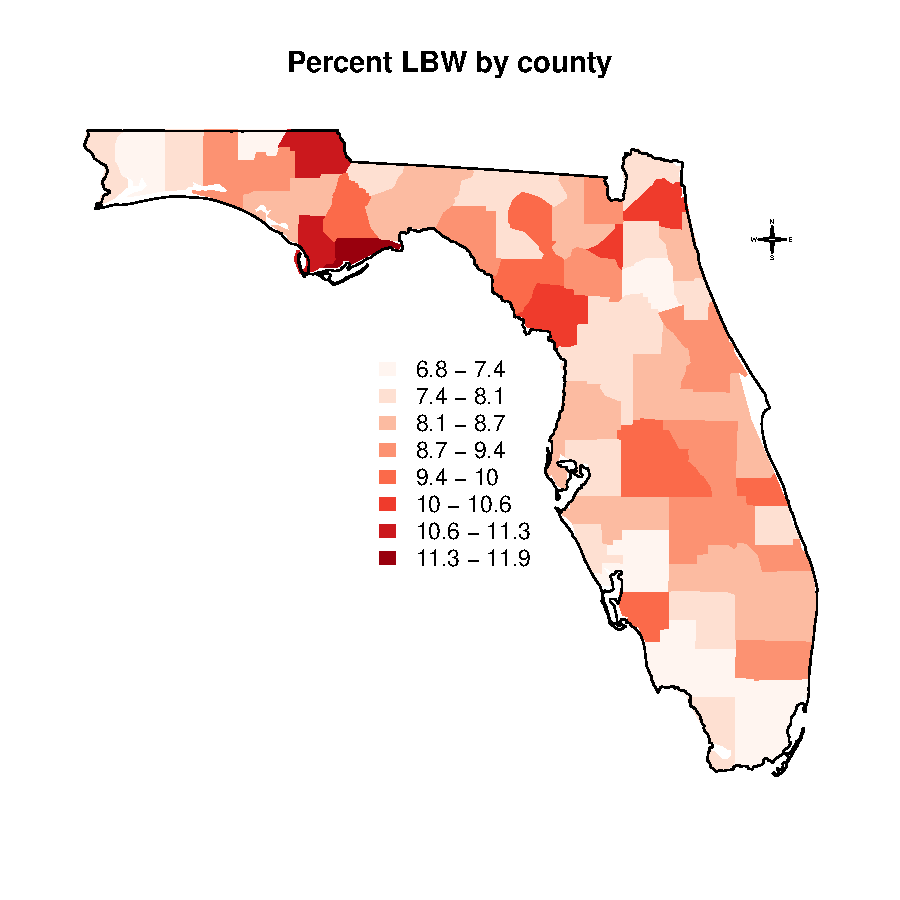
\includegraphics{final_project_proposal_joe_brew-001}

%------------------------------------------
\subsection*{Proposed methods}
\addcontentsline{toc}{subsection}{Proposed methods}
%------------------------------------------
Using individual-level data from the Florida Department of Health and WIC programs, I will construct geographic features (proximity to road, proximity to school, population density of census tract, county poverty rate, etc.) to supplement those already in the dataset (mother's age, birthweight, smoking status, etc.).  I will use logistic regression to predict a birth outcome (LBW or not) based on the spatial and sociodemographic predictors.  I will build my model on historical data (2006-2013) and test it on current data (2014), mapping residuals so as to identify system failings and missing predictors.  If applicable, I will employ general additive models with geographic smoothing and kriging so as to interpolate areal risks in the absence of an observation.






\end{multicols}
\setkeys{Gin}{width=1\textwidth}
%----------------------------------------------------------------------------------------
%  REFERENCE LIST
%----------------------------------------------------------------------------------------
\newpage
\bibliographystyle{unsrtnat}
\bibliography{test}


\end{document}
